\chapter{Convolutional Neural Networks} % Simulation results
\label{appx:simulation}

Convolutional Neural Networks for image classification \cite{krizhevsky2012imagenet} take image as an input, process it, and output category to which that image belongs. Processing part consists of a series of layers through which image is propagated in order to learn features, which in turn determine to which class an image belongs. (\textcolor{red}{\autoref{fig:cnn1}}).

\begin{figure}[h]
	\centering
	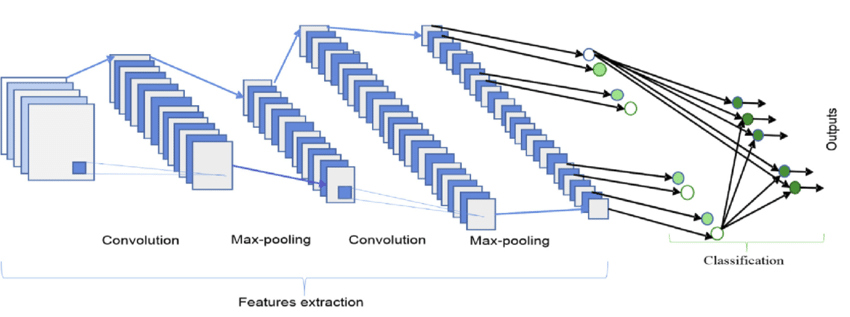
\includegraphics[scale=0.2]{cnn.png}
	\caption{Convolutional Neural Network consisting of two Convolution layers, two Max-Pooling layers, Flatten layer and two Fully-Connected (Dense) layers}
	\label{fig:cnn1}
\end{figure}

Most commonly used layers in CNN architectures are convolution layer, max-pooling layer, flatten layer, dense layer and dropout layer.

\subsection{Convolution Layer}

Convolution layer is the building block of the CNN architecture. Its primary purpose is to extract features from input image, such as edges, lines, curves, colors. As we go deeper inside the network, it starts identifying more complex features, such as shapes, objects. This layer consists of multiple filters (feature maps, usually 3x3 matrices) whose parameters need to be learned.
\subsection{Max-Pooling Layer}

Max-Pooling layer is located after a series of convolution layers in CNN architecture. It is a downsampling method which reduces dimensionality, thus decreasing number of parameters and computational power needed in order to train the network, while retaining important features and patterns. It is achieved by applying a max filter to non-overlapping subregions (usually 2x2 matrices), thus reducing the size of each feature map by a factor of 2.

\subsection{Flatten Layer}

Output of the convolutional base of the network (series of convolution and max-pooling layers) is a two-dimensional matrix, and before feeding that data to the classification top of the network, it needs to be transformed. Flatten layer reshapes the output matrix to vector, thus removing all dimensions but one in the process, making the data prepared for the series of fully-connected layers.

\subsection{Fully-Connected Layer}

After the high-level features of the image have been detected, series of fully-connected (dense) layers is attached to the top of the network in order to classify image into a label. Dense layers consist of huge number of nodes (neurons), which provide a way of learning non-linear combinations of features outputted by convolutional base, and determine which feature most correlate to a particular class.

\subsection{Dropout Layer}

Fully-Connected layer contains the most parameters in the network, and as a result neurons develop co-dependency amongst each other during training, which leads to overfitting the data (not generalizing well on new, unseen images). In order to prevent that, dropout layers are positioned right after dense layers in CNN architecture as a means of regularizing the network. Dropout consists of randomly ignoring (dropping out) fraction of neurons of fully-connected layer, which in turn makes network learn more robust features, and achieve better performance.
\clearpage
